\documentclass[14pt]{beamer}
\title[CP01.13 BC]{COJ :: Basics of Collections}
\author[TS]{TalentSprint}
\institute[L\&D]{Licensed To Skill}
\date{Version 1.0.4}
\usefonttheme{serif}
\usecolortheme{orchid}
\usepackage{bookman}
\usepackage{hyperref}
\usepackage[T1]{fontenc}
\usepackage{graphicx}
\usepackage{listings}
\graphicspath{{../../Images/}}
\lstset{language=Java,numbers=left, numberstyle=\tiny, basicstyle=\footnotesize, numbersep=10pt, showstringspaces=false, breaklines=true,keepspaces=true, columns=flexible}
\beamertemplateballitem
\usebackgroundtemplate{
\includegraphics[width=\paperwidth]{TS-Logo.jpg}}

\begin{document}
\begin{frame}
  \titlepage
\end{frame}
\begin{frame}{Collection Framework}
The content in this presentation is aimed learners to learn:
 \begin{itemize}
  \item Define collections 
  \item Understanding the importance of collections
  \item Identifying core collection interfaces and their implementation classes. 
  \item Perform basic operations on all collections
 
 \end{itemize}
\end{frame}

\begin{frame}{Collection Framework}
Java Collections Framework
\begin{itemize}
\item A Collection is a structured group of objects manipulate as a single object. Corresponds to a bag.
\end{itemize}
Limitations of Static Array
\begin{itemize}
\item Arrays are fixed size.
\item An array can only hold one type of objects (including primitives).
\end{itemize}
Example: Employee[] emp = new Employee[10];

\textbf{Note}  So we need Dynamic Arrays.
\end{frame}
\begin{frame}{Collection Framework}
\begin{itemize}
\item Collections are dynamic in nature and can grow as necessary.
\item Collections are Heterogeneous, can store different objects as part of a collection.
\item Collections can contain only Objects (reference types) and not primitives.
\item Collections are defined in java.util package
\end{itemize}
\end{frame}

\begin{frame}{Collection Framework}
Collection interfaces
\begin{center}
    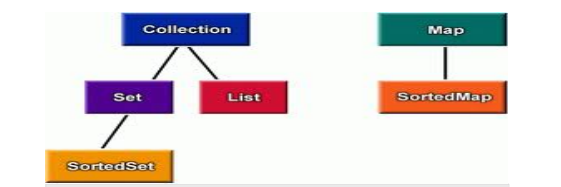
\includegraphics[scale=0.5]{COJ-M04-S01-Image1.png}
  \end{center}
\begin{itemize}
\item Collections are primarily defined through a set of interfaces.
\item As they are interfaces they do not provide any implementation
\item They are supported by a set of classes that implement the interfaces
\end{itemize}
\end{frame}

\begin{frame}{The Set Interface}
Corresponds to the mathematical definition of a set 
\begin{itemize}
\item No duplicates elements are allowed
\item No ordering of elements.
\item Indexing is not there
\end{itemize}
Set implementation classes are: \\
\textbf{HashSet:}
\begin{itemize}
\item Implemented using a hash table.
\item No ordering of elements.
\end{itemize}

\textbf{TreeSet:}
\begin{itemize}
\item Implemented using a tree structure.
\item Guarantees ordering of elements.
\end{itemize}
\end{frame}

\begin{frame}{The Set Interface}
\begin{description}
\item [add(Object) :] Adds the specified element to this set if it is not already present 
\item [remove(Object) :] Removes the specified element from this set if it is present
\item [size() :] Returns the number of elements in this set 
\end{description}
\end{frame}
\begin{frame}{The Set Interface}
\begin{description}
\item [contains(Object) :] Returns true if this set contains the specified element.
\item [containsAll(Collection) :] Returns true if this set contains all of the elements of the specified collection.
\item [retainAll(Collection) :] Retains only the elements in this set that are contained in the specified collection 
\end{description}
\end{frame}
\begin{frame}{Collection Framework}
HashSet Example
\begin{center}
    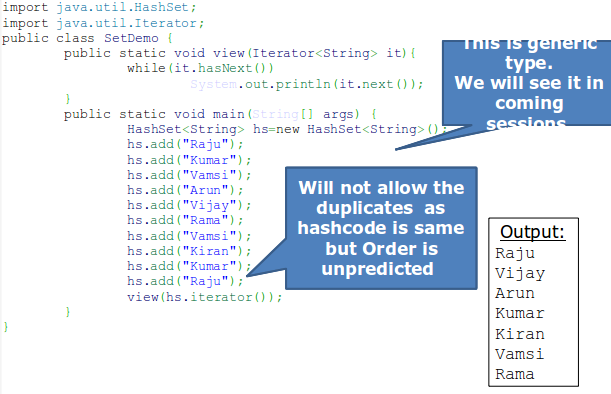
\includegraphics[scale=0.5]{COJ-M04-S01-Image2.png}
  \end{center}
\end{frame}

\begin{frame}{The List Interface}
The List interface corresponds to an order group of elements.
\begin{itemize}
\item Duplicates elements are allowed
\item Insertion ordering is maintained for elements.
\item Access to elements via indexes, like arrays
\end{itemize}
\end{frame}
\begin{frame}{The List Interface}
List implementation classes are:
\textbf{ ArrayList :}
\begin{itemize}
\item Its an array based implementation 
\item Elements can be accessed directly via the get and set methods using indexes.
\end{itemize}

\textbf{LinkedList:}
\begin{itemize}
\item Its a double linked list implementation.
\item Gives better performance on add and remove operations when compared to ArrayList
\end{itemize}
\end{frame}


\begin{frame}{Important methods of List interface:}
\begin{description}
\item [add(Object) :] adds element at the end of the list.
\item [add(index, Object) :] adds element at the specified index position.
\item [remove(Object) :] Removes the first occurrence of the specified element
\end{description}
\end{frame}
\begin{frame}{Important methods of List interface:}
\begin{description}
\item [indexOf(Object) :] Returns the index of the first occurrence of the specified element 
\item [get(index) :] Returns the element at the specified position in this list.
\item [set(index, Object) :] Replaces the element at the specified position in this list.
\end{description}
\end{frame}
\begin{frame}{The Map Interface}
\begin{itemize}
\item A Map is an object that maps keys to values
\item Keys are unique, values can be duplicated
\item A key is an object used to retrieve a value in Map
\item Map does not extend Collection interface
\end{itemize}
\end{frame}
\begin{frame}{The Map Interface}
Map implementation classes are: \\
\textbf{HashMap:}

\begin{itemize}
\item The implementation is based on a hash table.
\item No ordering on (key, value) pairs.
\end{itemize}
\textbf{TreeMap:}

\begin{itemize}
\item The implementation is based on tree structure.
\item (key, value) pairs are ordered on the key.
\end{itemize}
\end{frame}

\begin{frame}{Important methods of List interface:}
\begin{description}
\item [put(Object key, Object value) :] Associates the specified value with the specified key in this map.
\item [get(Object key) :] Returns the value to which the specified key is mapped.
\item [remove(Object Key) :] Removes the mapping for a key from this map if it is present.
\end{description}
\end{frame}

\begin{frame}{Important methods of List interface:}
\begin{description}
\item [keySet() :] Returns a Set view of the keys contained in this map.
\item [values() :] Returns a Collection view of the values contained in this map.
\end{description}
\end{frame}


\begin{frame}{Collection Framework}
\begin{center}

\includegraphics[scale=0.4]{COJ-M01-S03-Image27.png}
\end{center}
\end{frame}
\end{document}

